\documentclass[12pt,a4paper]{article}
\usepackage[utf8]{inputenc}
\usepackage[english]{babel}
\usepackage{csquotes}
\usepackage{amsmath, amsfonts, amssymb, array}
\usepackage{graphicx, subcaption}
\usepackage{setspace}
\usepackage{multicol}
\usepackage{parskip}
\setlength{\parindent}{4em}
\usepackage{fancyhdr}
\usepackage{hyperref}
\usepackage{pgfplots}
\pgfplotsset{compat=newest}% use newest version
\usepackage{tikz, tikz-3dplot,  circuitikz}
\usepackage{xcolor}
\usepackage{sectsty}
\usepackage{xstring}
\usepackage{caption}
\usepackage{listings}
\usepackage{biblatex}
\addbibresource{citations.bib}
\usepackage{dirtytalk}
\usepackage{units}

\definecolor{blu1}{HTML}{5DA2D5}
\definecolor{blu2}{HTML}{206B99}
\definecolor{lightblu}{HTML}{90CCF4}
\definecolor{red1}{HTML}{F78888} % <- darker 
\definecolor{red2}{HTML}{EDB5BF}  % sim to #ecb4b4, triadic colour of grn1
\definecolor{plumb}{HTML}{A16E83}
\definecolor{lilacc}{HTML}{86B3D1}
\definecolor{gren1}{HTML}{b4ecb4}


\usetikzlibrary{positioning}

\begin{document}
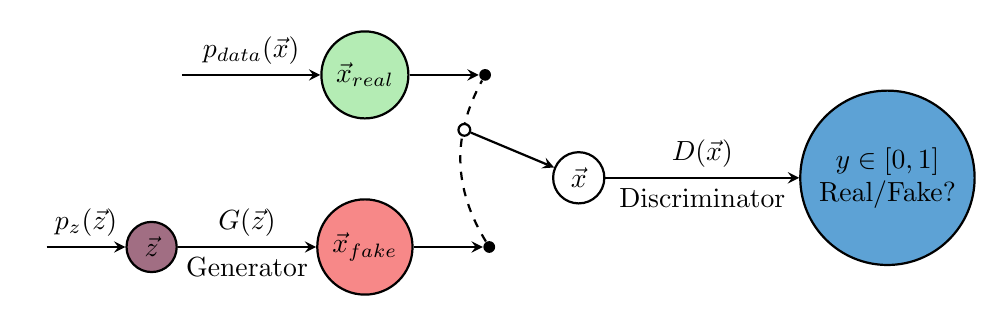
\begin{tikzpicture}

	\node[circle, draw, thick, fill=plumb] (z) {$\vec{z}$};
	\node[circle, draw, thick, right=5em of z, fill = red1] (x) {$\vec{x}_{fake}$};
	\draw[-stealth, thick ] (z) -- node[above] {$G(\vec{z})$} node[below] {Generator} (x);
	\node[left=of z] (i) {};
	\draw[-stealth, thick ] (i) -- node[above] {$p_z(\vec{z})$} (z);
	\node[above=of x, circle, draw, thick, fill = gren1] (xt) {$\vec{x}_{real}$};
	\node[left=5em of xt] (it) {};
	\draw[-stealth, thick] (it) -- node[above] {$p_{data}(\vec{x})$} (xt) ;
	\node[circle, draw, thick, right=5em of x, yshift=2.5em] (D) {$\vec{x}$};
	\node[circle, draw,  thick, right=7em of D, fill = blu1, align=center] (out) {$y\in [0,1]$ \\ Real/Fake?};
	\draw[-stealth, thick] (D) -- node[above] {$D(\vec{x})$} node[below] {Discriminator} (out);
			
	\node[right=2.5em of x, circle, fill, inner sep=0.15em] (pt1) {};
	\node[right=2.5em of xt, circle, fill, inner sep=0.15em] (pt2) {};
			
	\draw[dashed, thick] (pt1) edge[bend left] (pt2);
			
	\node[circle, draw, thick, fill=white, inner sep=0.15em] at ([xshift=-0.9em, yshift=4em]pt1.north) (pt3) {};
			
	\draw[-stealth, thick] (x) -- (pt1);
	\draw[-stealth, thick] (xt) -- (pt2);
	\draw[-stealth, thick] (pt3) -- (D);

\end{tikzpicture}





\begin{tikzpicture}[ampersand replacement=\&]
%     \draw[help lines](0,-5) grid (10,5);  
     
   	\node[text width=1.75cm] at (-3,0) (Z) {\textsc{Random Noise ($ \mathbf{z} $)}};		 
    \node[rectangle, rounded corners, draw, fill=blue!20, minimum height=1cm] at (0,0) (G) {\textsc{Generator}};	
    \node[rectangle, rounded corners, draw, fill=cyan!20, minimum height=1cm] at (3,0) (S1) {\textsc{Sample}};
    
    \node[text width=1.75cm] at (0.5,3) (X) {\textsc{Training Data ($ \mathbf{x} $)}};		 
    \node[rectangle, rounded corners, draw, fill=cyan!20, minimum height=1cm] at (3,3) (S2) {\textsc{Sample}};
    
    \node[rectangle, rounded corners, draw, fill=red!20, minimum height=1cm] at (6,1.5) (D) {\textsc{Discriminator}};
    
    \node[text width=2cm] at (10,1.5) (O) {\textsc{Real/Fake Prediction}};
     
    \path[arrow] (Z) edge (G)
    (G) edge (S1)
    (S1) edge (D.south west)
    (X) edge (S2)
    (S2) edge (D.north west)  
    (D) edge (O)
    ;
\end{tikzpicture}



\end{document}